\subsubsection{Listar}

  \paragraph{}Para mostrar esta lista, es necesario establecer el centro para
  el que mostrar las asignaturas curso académico disponibles. Para ello, habrá
  que elegir el centro en la lista desplegable que se muestra en la figura
  \ref{capturaPantallaSelectCentro}.

  \paragraph{}También será necesario elegir la titulación a la que pertenecen
  las asignaturas, por lo que se elegirá entre las opciones de una lista
  desplegable, siguiendo el mismo mecanismo que para seleccionar centro. Se
  puede ver una captura de la selección de titulación en la figura
  \ref{capturaPantallaSelectTitulacion}.

  \paragraph{}Por último, habrá que seleccionar la asignatura para la cual se
  listarán los cursos académicos disponibles. Al igual que para la selección de
  centro y de titulación, se seleccionará a través de una lista desplegable con
  las asignaturas disponibles. La figura \ref{capturaPantallaSelectAsignatura}
  muestra una captura de pantalla de esta ventana.

  \begin{figure}[!ht]
    \begin{center}
      \fbox{
      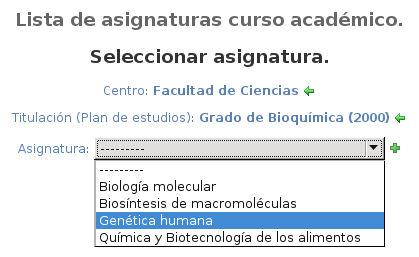
\includegraphics[scale=0.55]{4.Funcionamiento_Aplicacion/4.3.Gestion/4.3.1.Administrador_Principal/4.3.1.7.AsignaturaCA/select_asignatura.png}
      }
      \caption{Captura de pantalla de la lista desplegable para seleccionar asignatura para el usuario \textit{Administrador principal}.}
      \label{capturaPantallaSelectAsignatura}
    \end{center}
  \end{figure}

  \paragraph{}Nótese que si no existieran elementos disponibles en el sistema,
  la lista desplegable aparecería vacía. Por tanto, se proporciona al usuario
  un icono, representado por una cruz verde, para añadir nuevos elementos al
  sistema. Este icono es el mostrado en la figura \ref{capturaBotonAdd}. Al
  pulsar dicho botón, aparecerá la ventana de creación de un nuevo elemento.

  \paragraph{}Una vez seleccionados el centro, la titulación y la asignatura, se
  muestra la lista completa de asignaturas curso académico que aparecen en el
  sistema. La figura \ref{capturaPantallaListaAsignaturasCAAdminPrincipal}
  muestra una captura de pantalla de la lista de asignaturas curso académico.

  \begin{figure}[!ht]
    \begin{center}
      \fbox{
      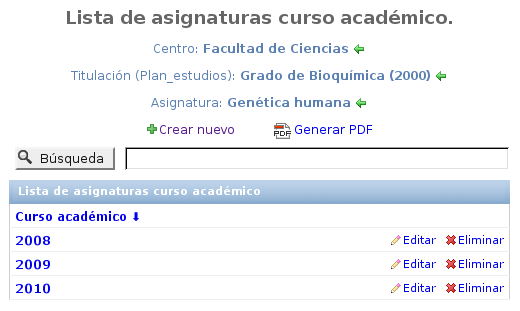
\includegraphics[scale=0.55]{4.Funcionamiento_Aplicacion/4.3.Gestion/4.3.1.Administrador_Principal/4.3.1.7.AsignaturaCA/lista_asignaturasCA.png}
      }
      \caption{Captura de pantalla de la lista de asignaturas curso académico para el usuario \textit{Administrador principal}.}
      \label{capturaPantallaListaAsignaturasCAAdminPrincipal}
    \end{center}
  \end{figure}

  \paragraph{}Si se quisiera refinar el listado de elementos mostrados, es
  posible seleccionar nuevos parámetros pulsando el icono \textit{Seleccionar}
  que aparece al lado de cada elemento. Este icono aparece en la figura
  \ref{capturaBotonSeleccionar}.
